\documentclass[12pt, fleqn]{article}

\usepackage[utf8]{inputenc}
\usepackage[T2A]{fontenc}
\usepackage{amssymb, amsmath, mathrsfs, amsthm}
\usepackage[russian]{babel}
\usepackage{graphicx}
\usepackage[footnotesize]{caption2}
\usepackage{indentfirst}
\usepackage[hidelinks]{hyperref}
\usepackage{multirow}
%\usepackage[ruled,section]{algorithm}
%\usepackage[noend]{algorithmic}
%\usepackage[all]{xy}

% Параметры страницы
\textheight=24cm
\textwidth=16cm
\oddsidemargin=5mm
\evensidemargin=-5mm
\marginparwidth=36pt
\topmargin=-1cm
\footnotesep=3ex
%\flushbottom
\raggedbottom
\tolerance 3000
% подавить эффект "висячих стpок"
\clubpenalty=10000
\widowpenalty=10000
\renewcommand{\baselinestretch}{1.1}
\renewcommand{\baselinestretch}{1.5} %для печати с большим интервалом

% Дополнительные команды для личных обозначений
\newcommand{\expectation}{\mathop{\mathbb{E}}}
\newcommand{\norm}[1]{\left\lVert#1\right\rVert}
\newcommand{\loss}{\mathop{\mathcal{L}}}
\newcommand{\mse}{\mathop{MSE}}
\newcommand{\scalarproduct}[1]{\langle #1 \rangle}

\newcommand{\predictionfunction}{\hat{f}}
\newcommand{\ensemblefunction}{a}
\newcommand{\optimizationmethodfunction}{\tilde{f}}
\newcommand{\distinguishparameter}{\alpha}
\newcommand{\objects}{X}
\newcommand{\results}{Y}
\newcommand{\predictedobjects}{\widehat{\objects}}

\newcommand{\numberobjects}{N}
\newcommand{\numberpredictionfunctions}{M}

\newcommand{\for}[3]{\sum\limits_{#1 = #2}^{#3}}  % Usage: \for{index}{begin}{end}
\newcommand{\forn}[2]{\for{#1}{1}{#2}}  % Usage: \forn{index}{end}

\newcommand{\many}[3]{#1 1 #2, #1 2 #2, \dots, #1 #3 #2}  % Usage: \many{prefix}{suffix}{end}

\newcommand{\reference}[1]{(\hyperref[#1]{\ref{#1}})}

\newcommand{\ensemblefunctionfull}{\ensemblefunction(\many{\predictionfunction_}{(x)}{\numberpredictionfunctions})}

\begin{document}
	
	\begin{titlepage}
		\begin{center}
			Московский государственный университет имени М. В. Ломоносова
			
			\bigskip
			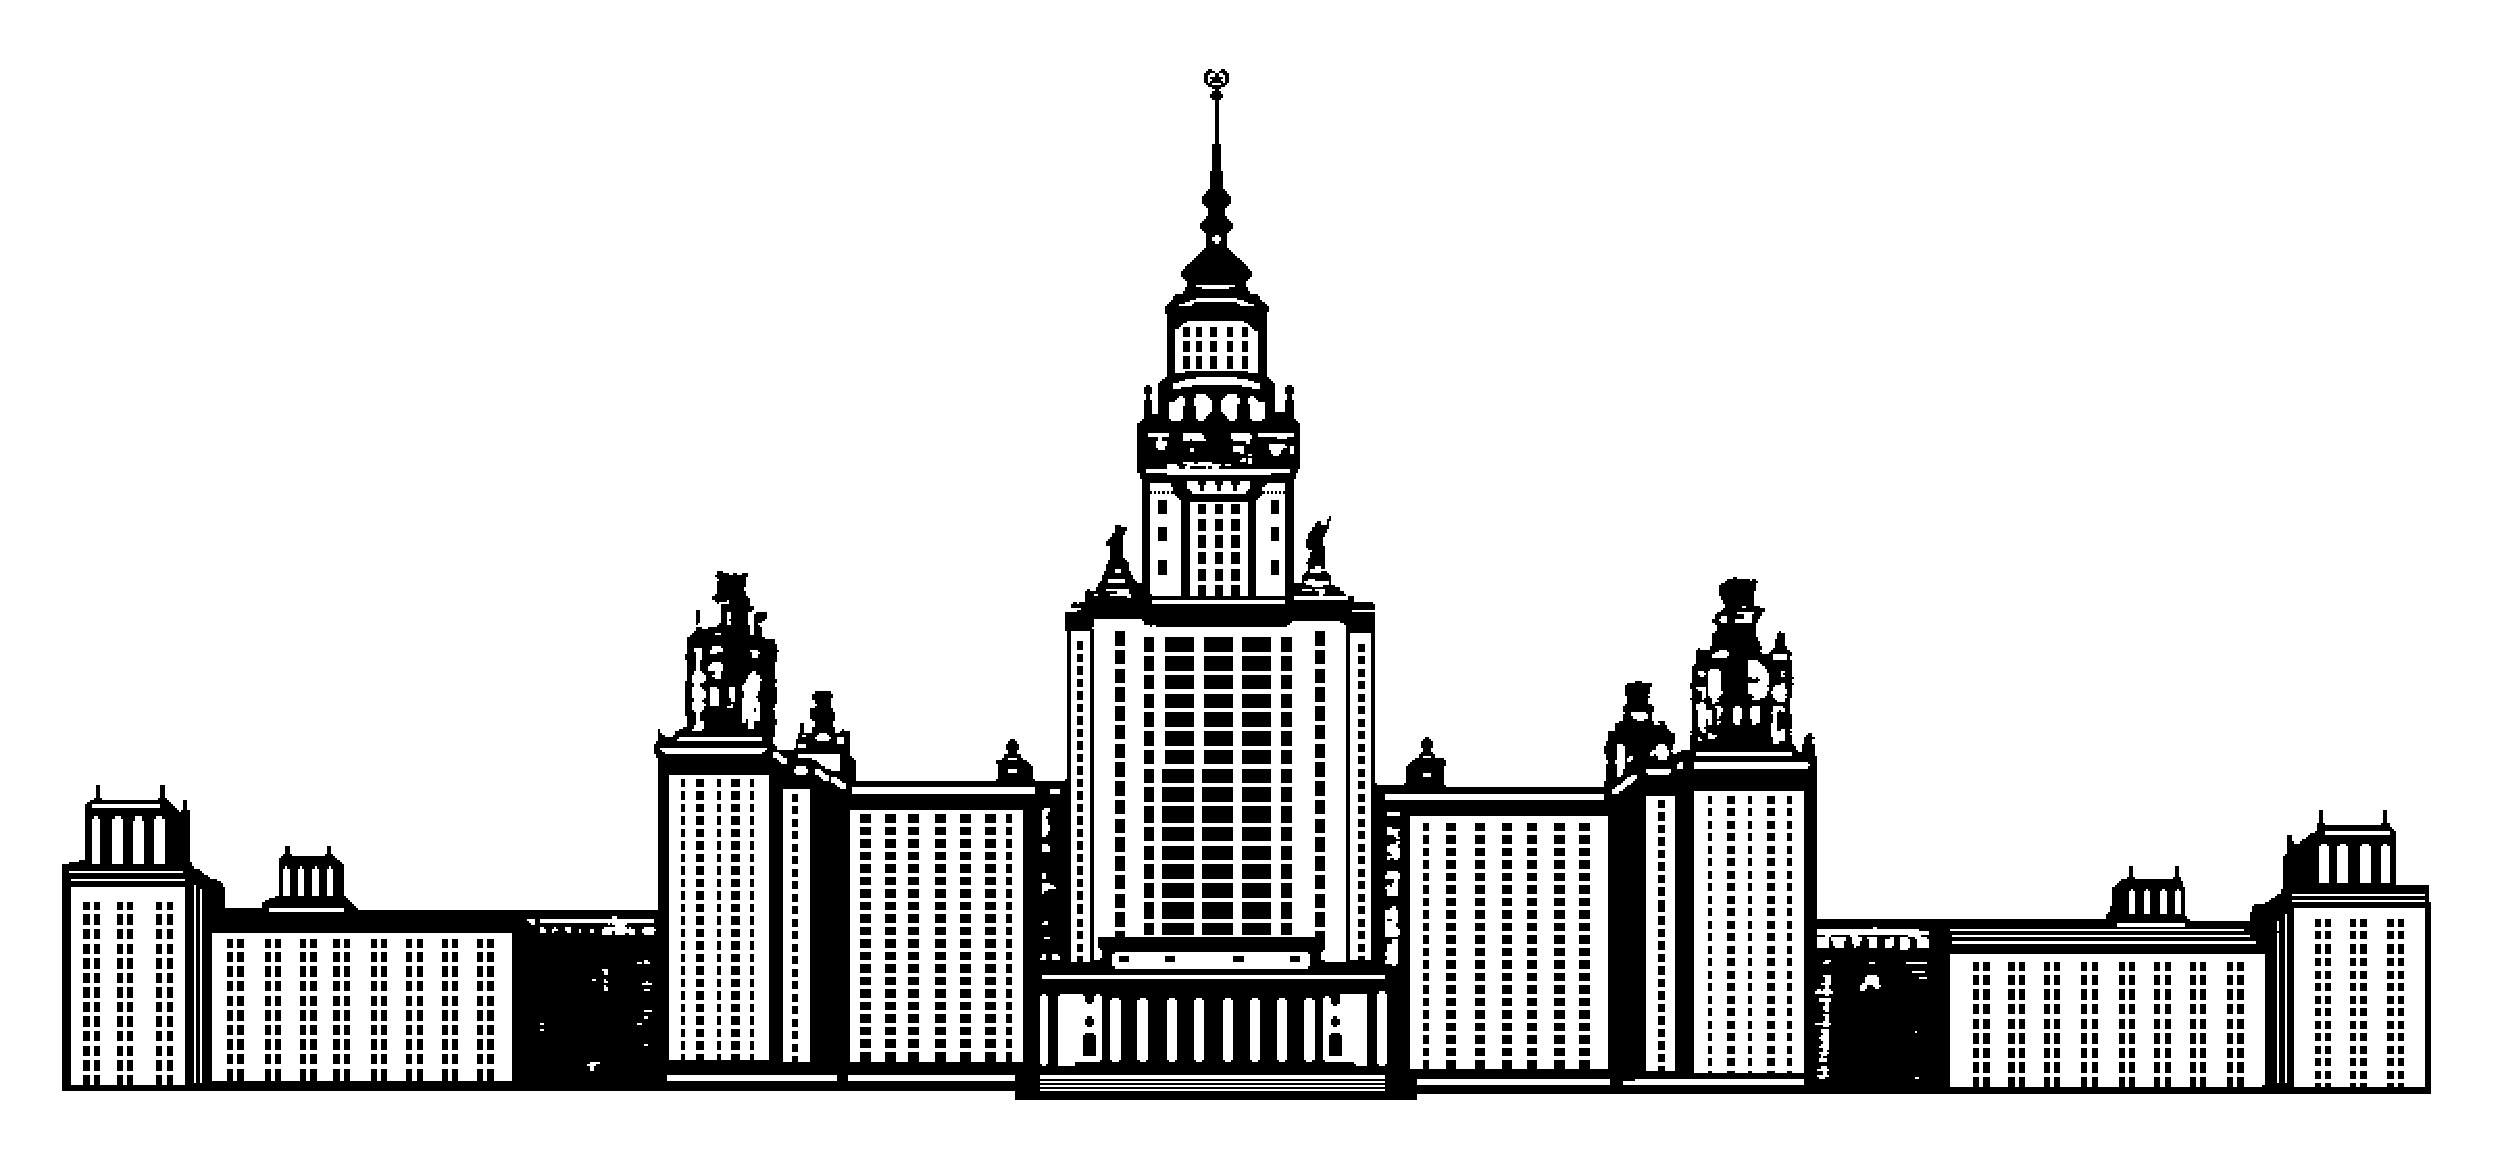
\includegraphics[width=50mm]{msu.eps}
			
			\bigskip
			Факультет Вычислительной Математики и Кибернетики\\
			Кафедра Математических Методов Прогнозирования\\[10mm]
			
			\textsf{\large\bfseries
				КУРСОВАЯ РАБОТА\\[10mm]
				<<Исследование методов аугментации аудиоданных>>\\
				<<Research of audio data augmentation methods>>
			}\\[10mm]
			
			\begin{flushright}
				\parbox{0.5\textwidth}{
					Выполнил:\\
					студент 5 курса 517 группы\\
					\emph{Лукьянов Павел Александрович}\\[5mm]
					Научный руководитель:\\
					д.ф-м.н., профессор\\
					\emph{Дьяконов Александр Геннадьевич}
				}
			\end{flushright}
			
			\vspace{\fill}
			Москва, 2021
		\end{center}
	\end{titlepage}
	
	\newpage
	\renewcommand{\contentsname}{Содержание}
	\tableofcontents
	
	\newpage
	\begin{abstract}
		В данной работе исследуются методы аугментации звуковых данных. На двух задачах аудиоклассификации проверяется эффективность как давно известных методов аугментации, так и предложенных в данной работе подходов. Результаты экспериментов показывают перспективность некоторых из предложенных методов.
	\end{abstract}
	
	\newpage
	\section{Введение}
	
	Исследование методов аугментации очень актуально в настоящее время. Понятию аугментации сложно дать точное определение, в данной работе под ней будем понимать создание новых данных на основе уже имеющихся. С помощью аугментации можно существенно расширить объем обучающей выборки, что особенно хорошо в тех случаях, когда исходных данных не очень много. Применение аугментации способно повысить обобщающую способность модели. 
	
	Аугментация данных используется при решении многих задач глубинного обучения, связанных с обработкой изображений, текстов, звуковых данных. Классическим примером задачи, в которой используется аугментация, является задача классификации ~\cite{b2}, ~\cite{b3}. Применение аугментации позволяет добиться лучшего качества в задаче автоматического распознавания речи ~\cite{b1}. 
		
	В данной работе будем исследовать применение методов аугментации в задаче аудиоклассификации. Соответственно, аугментация будет применяться к звуковым данным, а именно к мел-спектрограммам ~\cite{b1}, которые, в свою очередь, будут подаваться на вход нейронной сети как изображения. 
	
	Обычная спектрограмма получается после применения оконного преобразования Фурье к коротким кускам речевого сигнала. После же применения мел-фильтров к этой спектрограмме и получается мел-спектрограмма ~\cite{b8}, в которой частота выражена в мелах.
	
	В данной работе мел-спектрограммы нормализуются следующим образом: 
	
	$ value = \frac{value - mean}{std}$, где mean -- математическое ожидание значений мел-спектрограммы, std -- стандартное отклонение. 
	
	Такая нормализация, в частности, важна для корректного обоснования некоторых методов аугментации, описанных в следующих разделах.
	\section{Существующие методы аугментации}
	В этом разделе представлены известные методы аугментации аудиоданных, которые будем исследовать и на основе которых будут предложены некоторые из новых подходов. 	
	\newline Здесь и далее считаем, что FreqSize -- размерность мел-спектрограммы по частотной оси, TimeSize -- размерность мел-спектрограммы по временной оси.
	$S$ -- матрица значений мел-спектрограммы. \newline
	Также введем матрицу $M(I, J)$, где $I, J$ - множества индексов: \newline 
	\begin{equation*}
	M(I, J) = \{M(i, j)\} = 
	\begin{cases}
	0, & (i,j) \in I \times J,\\
	1, &\text{иначе}.
	\end{cases}
	\end{equation*}
	Стоит рассматривать только случаи, когда в представленных ниже аугментациях значения $t$, $f$, shift ненулевые. В противном случае ($t = 0$, или $f = 0$, или shift = 0) мел-спектрограмма никак не изменяется.
	
	\begin{enumerate}
		\item TimeMasking \ref{fig:i5}. ~\cite{b1} \newline 
		$t \sim U\{0, T\}, t_0 \sim U\{0, \text{TimeSize} - 1 - t\}$, $T$ - параметр аугментации. \newline 
		В результате применения аугментации: \newline
		$S \rightarrow S \cdot M(\{0, \ldots, \text{FreqSize} - 1\}, \{t_0, \ldots, t_0 + t - 1\}) $
		\begin{figure}[h]
			\center{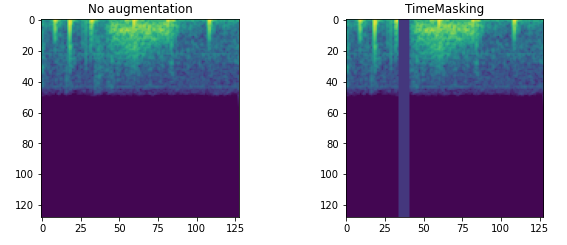
\includegraphics[scale=0.9]{5.png}}
			\caption{TimeMasking}
			\label{fig:i5}
		\end{figure}
		\item FreqMasking \ref{fig:i6}. ~\cite{b1} \newline
		$f \sim U\{0, F\} f_0 \sim U\{0, \text{FreqSize} - 1 - f\}$, $F$ - параметр аугментации. \newline
		В результате применения аугментации: \newline
		$S \rightarrow S \cdot M(\{f_0, \ldots, f_0 + f - 1\}, \{0, \ldots, \text{TimeSize} - 1\}) $
		\begin{figure}[h]
			\center{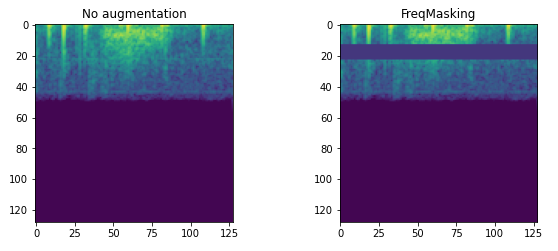
\includegraphics[scale=0.9]{6.png}}
			\caption{FreqMasking}
			\label{fig:i6}
		\end{figure}
		\item Noise \ref{fig:i7}. ~\cite{b2} \newline 
		К каждому значению в мел-спектрограмме добавляется $g \sim N(0, \sigma)$ (для каждого значения мел-спектрограммы генерируется свое g), где $\sigma$ - параметр аугментации (в данной работе $\sigma = 0.01$). 
		\begin{figure}[h]
			\center{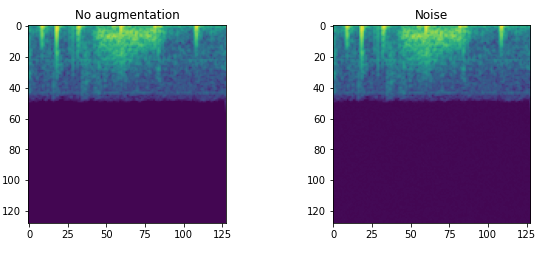
\includegraphics[scale=0.9]{7.png}}
			\caption{Noise}
			\label{fig:i7}
		\end{figure}
		\item TimeShift \ref{fig:i8}. ~\cite{b2} \newline Сдвигаем все значения мел-спектрограммы относительно временной оси влево или вправо на |shift|, где $\text{shift} \sim U\{-\text{max\_shift}, \text{max\_shift}\}$, max\_shift - параметр аугментации. Направление сдвига определяется знаком shift: если \newline shift > 0, происходит сдвиг вправо, если shift < 0 - влево. Пустая область, образующаяся в результате сдвига, заполняется нулями.
		\begin{figure}[h]
			\center{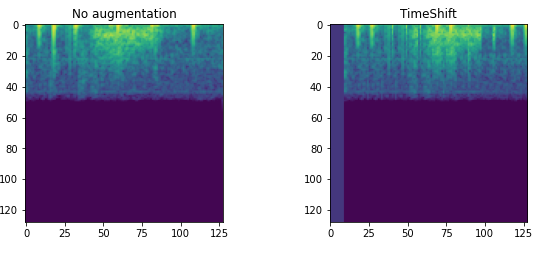
\includegraphics[scale=0.9]{8.png}}
			\caption{TimeShift}
			\label{fig:i8}
		\end{figure}
		\item RandomErasing \ref{fig:i9}. ~\cite{b3} Случайное вырезание прямоугольника в мел-спектрограмме. \newline
		$t \sim U\{0, T\}, t_0 \sim U\{0, \text{TimeSize} - t - 1\}$, \newline $f \sim U\{0, F\}, f_0 \sim U\{0, \text{FreqSize} - f - 1\}$, $T, F$ - параметры аугментации. \newline
		В результате применения аугментации: \newline
		$S \rightarrow S \cdot M(\{f_0, \ldots, f_0 + f - 1\}, \{ t_0, \ldots, t_0 + t - 1\}) $
		\begin{figure}[h]
			\center{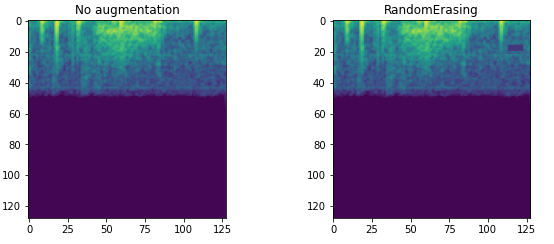
\includegraphics[scale=0.9]{9.png}}
			\caption{RandomErasing}
			\label{fig:i9}
		\end{figure}
	\end{enumerate}
	Стоит отметить, что в связи с нормализацией мел-спектрограммы замена некоторых значений на 0 в результате применения аугментации -- это замена на математическое ожидание ~\cite{b1}.
	\section{Предлагаемые подходы к аугментации}
	
	Ниже представлены предлагаемые возможные подходы к аугментации звуковых данных:
	
	\begin{enumerate}
		\item FreqShift \ref{fig:i10}. \newline Аналог TimeShift, только теперь сдвиг происходит относительно частотной оси. \newline
		$\text{shift} \sim U\{-\text{max\_shift}, \text{max\_shift}\}$, $\text{max\_shift}$ - параметр аугментации. Направление сдвига определяется знаком shift: если shift > 0, происходит сдвиг вниз, если shift < 0 - вверх. Пустая область, образующаяся в результате сдвига, заполняется нулями.
		\begin{figure}[h]
			\center{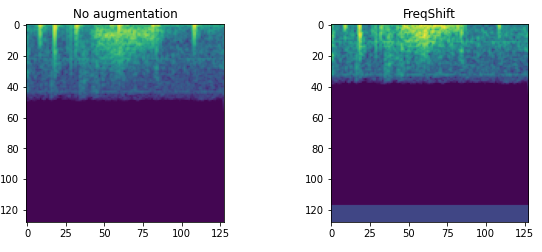
\includegraphics[scale=0.9]{10.png}}
			\caption{FreqShift}
			\label{fig:i10}
		\end{figure}
		\item ТimeNoising \ref{fig:i11}. \newline
		$t \sim U\{0, T\}, t_0 \sim U\{0, \text{TimeSize} - t - 1\}$, $T$ - параметр аугментации. \newline Ко всем  значениями мел-спектрограммы, индексы которых принадлежат множеству $\{0, \ldots, \text{FreqSize} - 1\} \times \{t_0, \ldots, t_0 + t - 1\}$, добавляется значение $g \sim N(0, \sigma)$ (для каждого значения мел-спектрограммы генерируется свое g), где $\sigma$ - параметр аугментации (в данной работе $\sigma = 0.1$). Идея метода заключается в том, чтобы зашумлять не всю мел-спектрограмму, а только отдельные ее участки.
		\begin{figure}[h]
			\center{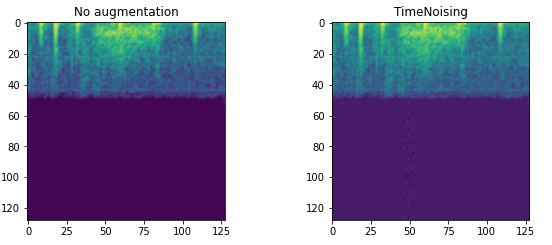
\includegraphics[scale=0.9]{11.png}}
			\caption{ТimeNoising}
			\label{fig:i11}
		\end{figure}
		\item FreqNoising \ref{fig:i12}. \newline
		$f \sim U\{0, F\}, f_0 \sim U\{0, FreqSize - f - 1\}$, $F$ - параметр аугментации. \newline Ко всем  значениями мел-спектрограммы, индексы которых принадлежат множеству $\{f_0, \ldots, f_0 + f - 1\} \times \{0, \ldots, \text{TimeSize} - 1\}$, добавляется значение \newline $g \sim N(0, \sigma)$ (для каждого значения мел-спектрограммы генерируется свое g), где $\sigma$ - параметр аугментации (в данной работе $\sigma = 0.1$).
		\begin{figure}[h]
			\center{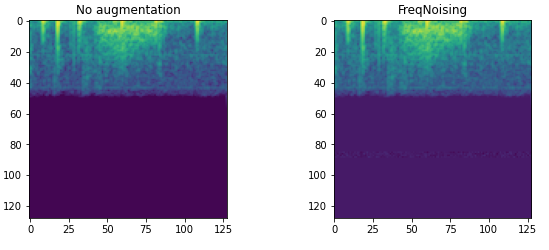
\includegraphics[scale=0.9]{12.png}}
			\caption{FreqNoising}
			\label{fig:i12}
		\end{figure}
		\item TimeCycleShift \ref{fig:i1}. \newline
		Циклический сдвиг всех значений мел-спектрограммы относительно временной оси влево или вправо на |shift|, где $\text{shift} \sim U\{-\text{max\_shift}, \text{max\_shift}\}$, max\_shift - параметр аугментации. Направление сдвига выбирается так же, как и в TimeShift.  
		\begin{figure}[h]
			\center{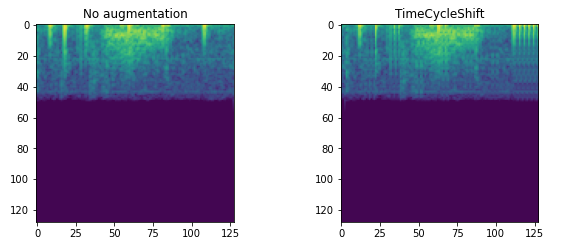
\includegraphics[scale=0.9]{1.png}}
			\caption{TimeCycleShift}
			\label{fig:i1}
		\end{figure}
		\item FreqCycleShift \ref{fig:i13}. \newline
		Циклический сдвиг всех значений мел-спектрограммы относительно частотной оси вверх или вниз на |shift|, где $\text{shift} \sim U\{-\text{max\_shift}, \text{max\_shift}\}$, max\_shift - параметр аугментации. Направление сдвига выбирается так же, как и в FreqShift.
		\begin{figure}[h]
			\center{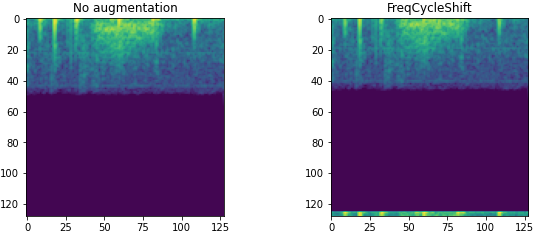
\includegraphics[scale=0.9]{13.png}}
			\caption{FreqCycleShift}
			\label{fig:i13}
		\end{figure}
		\item TimeSpecialShift \ref{fig:i14}. \newline
		Сдвиг всех значений мел-спектрограммы относительно временной оси влево или вправо на |shift|, где $\text{shift} \sim U\{-\text{max\_shift}, \text{max\_shift}\}$, max\_shift - параметр аугментации. Направление сдвига выбирается так же, как и в TimeShift. Пустая область, образующаяся в результате сдвига, заполняется значениями из исходной спектрограммы $S[0: \text{FreqSize} - 1; 0: |\text{shift}| - 1]$ в случае сдвига вправо или $S[0: \text{FreqSize} - 1;  \text{TimeSize} - |\text{shift}|: \text{TimeSize} - 1]$ в противном случае. Идея метода заключается в том, чтобы пустой участок, образующийся в результате сдвига, заполнять не нулями, а значениями из соседнего участка.
		\begin{figure}[h]
			\center{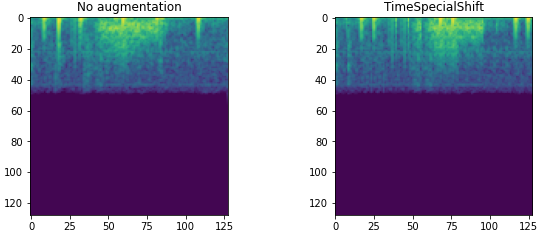
\includegraphics[scale=0.9]{14.png}}
			\caption{TimeSpecialShift}
			\label{fig:i14}
		\end{figure}
		\item FreqSpecialShift \ref{fig:i15}. \newline
		Сдвиг всех значений мел-спектрограммы относительно частотной оси вверх или вниз на |shift|, где $\text{shift} \sim U\{-\text{max\_shift}, \text{max\_shift}\}$, max\_shift - параметр аугментации. Направление сдвига выбирается так же, как и в FreqShift. Пустая область, образующаяся в результате сдвига, заполняется значениями из исходной спектрограммы $S[0: |\text{shift}| - 1; 0: \text{TimeSize} - 1]$ в случае сдвига вниз или \newline $S[\text{FreqSize} - |\text{shift}| : \text{FreqSize} - 1; 0: \text{TimeSize} - 1]$ в противном случае.
		\begin{figure}[h]
			\center{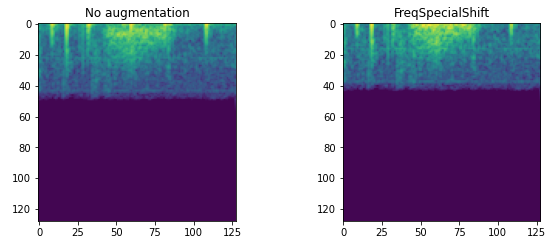
\includegraphics[scale=0.9]{15.png}}
			\caption{FreqSpecialShift}
			\label{fig:i15}
		\end{figure}
		\item TimeSwapAugmentation \ref{fig:i2}. \newline
		$t \sim U\{0, T\}, t_0 \sim U\{t, \text{TimeSize} - 1 - t\}$, $T$ - параметр аугментации. \newline
		В результате применения аугментации: \newline
	    $S[0:\text{FreqSize} - 1; t_0: t_0 + t - 1] \leftrightarrow S[0:\text{FreqSize} - 1; t_0 - t: t_0 - 1]$ \newline Идея метода заключается в перестановке соседних участков.
		\begin{figure}[h]
			\center{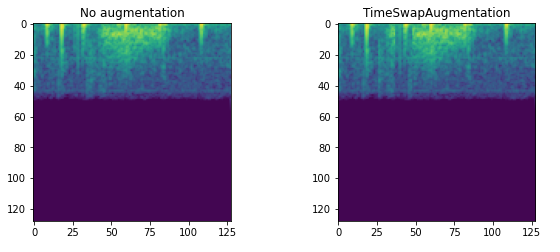
\includegraphics[scale=0.9]{2.png}}
			\caption{TimeSwapAugmentation}
			\label{fig:i2}
		\end{figure}
		
		\item FreqSwapAugmentation \ref{fig:i16}.
		$f \sim U\{0, F\}, f_0 \sim U\{f,\text{FreqSize} - 1 - f\}$, $F$ - параметр аугментации. \newline
		В результате применения аугментации: \newline
		$S[f_0: f_0 + f - 1; 0:\text{TimeSize} - 1] \leftrightarrow S[f_0 - f: f_0 - 1; 0:\text{TimeSize} -1]$ 
		\begin{figure}[h]
			\center{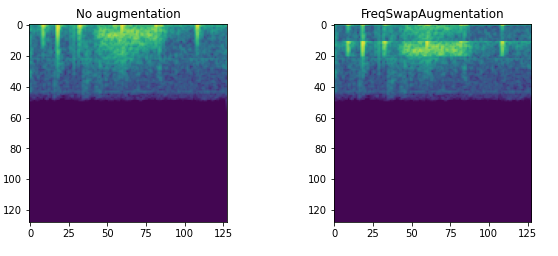
\includegraphics[scale=0.9]{16.png}}
			\caption{FreqSwapAugmentation}
			\label{fig:i16}
		\end{figure}
		\item ТimeReplyMasking \ref{fig:i4}. \newline
		$t \sim U\{0, T\}, t_0 \sim U\{t, \text{TimeSize} - 1 - 2 t\}$, $T$ - параметр аугментации. \newline Участок $S[0:\text{FreqSize} - 1; t_0: t_0 + t - 1]$ заменяется на один из участков \newline $S[0:\text{FreqSize} - 1, t_0 - t: t_0 - 1]$, $S[0:\text{FreqSize} - 1; t_0 + t: t_0 + 2 t -  1]$ в зависимости от направления. Направление выбирается с вероятностью 0.5. Идея метода похожа на идею в TimeSpecialShift.
			\begin{figure}[h]
			\center{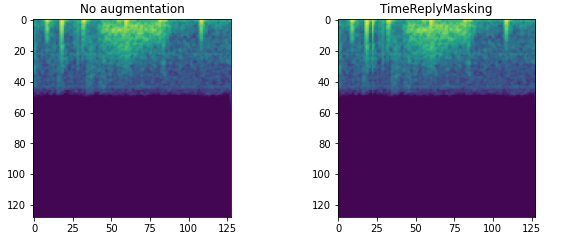
\includegraphics[scale=0.9]{4.png}}
			\caption{ТimeReplyMasking}
			\label{fig:i4}
		\end{figure}
		\item FreqReplyMasking \ref{fig:i17}. \newline
		$f \sim U\{0, F\}, f_0 \sim U\{f, \text{FreqSize} - 1 - 2 f\}$, $F$ - параметр аугментации. \newline Участок $[f_0: f_0 + f - 1; 0:\text{TimeSize} - 1]$ заменяется на один из участков \newline $[f_0 - f: f_0 - 1; 0:\text{TimeSize} - 1]$, $[f_0 + f: f_0 + 2 f - 1; 0:\text{TimeSize} - 1]$ в зависимости от направления. Направление выбирается с вероятностью 0.5.
		\begin{figure}[h]
			\center{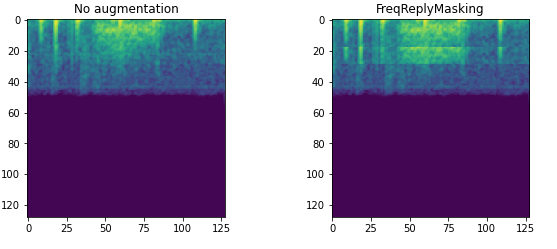
\includegraphics[scale=0.9]{17.png}}
			\caption{FreqReplyMasking}
			\label{fig:i17}
		\end{figure}
		\item TimeRandomSwap \ref{fig:i3}. \newline
		$t \sim U\{0, T\}, t_1 \sim U\{t, \text{TimeSize} - 1 - t\}, t_2 \sim U\{t, \text{TimeSize} - 1 - t\}, |t_1 - t_2| >= t $, $T$ - параметр аугментации. \newline 
		В результате применения аугментации: \newline
		$S[0:\text{FreqSize} - 1; t_1: t_1 + t - 1] \leftrightarrow S[0:\text{FreqSize} - 1; t_2 : t_2 + t - 1]$ \newline
		Идея метода заключается в перестановке произвольных участков.
		\begin{figure}[h]
			\center{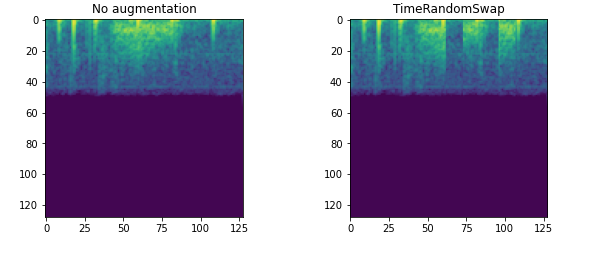
\includegraphics[scale=0.9]{3.png}}
			\caption{TimeRandomSwap}
			\label{fig:i3}
		\end{figure}
		\item FreqRandomSwap \ref{fig:i18}. \newline
		$f \sim U\{0, F\}, f_1 \sim U\{f, \text{FreqSize} - 1 - f\}, f_2 \sim U\{f, \text{FreqSize} - 1 - f\}, |f_1 - f_2| >= f $, $F$ - параметр аугментации. \newline 
		В результате применения аугментации: \newline
		$S[f_1: f_1 + f - 1; 0:\text{TimeSize} - 1] \leftrightarrow S[f_2 : f_2 + f - 1; 0:\text{TimeSize} - 1]$.
		\begin{figure}[h]
			\center{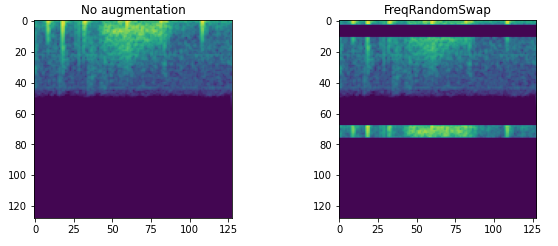
\includegraphics[scale=0.9]{18.png}}
			\caption{FreqRandomSwap}
			\label{fig:i18}
		\end{figure}
	\end{enumerate}

	\section{Вычислительные эксперименты}
	
	Методы аугментации будем анализировать применительно к задачам аудиоклассификации. Для этой цели будем использовать 2 набора данных: AudioMnist ~\cite{b7} и HeartBeatSounds ~\cite{b6}. 
	
	Датасет AudioMnist состоит из 3000 записей (файлов формата .wav), на которых некоторый человек произносит одну из 10 цифр. Соответственно, задача классификации заключается в том, чтобы определить какую конкретно цифру произносит человек на записи.
	
	Датасет HeartBeatSounds представляет собой записи звуков сердцебиения (656 файлов формата .wav). Задача - определить, к какому из 3 типов относятся звуки на записи: normal, murmur, extrastole.  
	
	В этих двух датасетах оставим только те записи, длина которых больше некоторого порогового значения. Из оставшихся файлов в каждом датасете извлекаем фиксированные по длине куски записи. Это необходимо для того, чтобы мел-спектрограммы были одного размера. 
	
	Для решения задач классификации будем использовать нейронные сети архитектур resnet18 и resnet50 и алгоритм оптимизации Adam. Нейронная сеть будет обучаться 75 эпох в случае AudioMnist и 70 эпох в случае HeartBeatSounds. Функция потерь - кросс-энтропия. 
	
	В данной работе значения параметров $F$ и $T$ для всех типов аугментаций, где используются эти параметры, считаем равными $0.1 \cdot \text{FreqSize} - 1$ и $0.1 \cdot \text{TimeSize} - 1$ соответственно. Параметр max\_shift будем считать равным $0.1 \cdot \text{FreqSize} - 1$ в случае сдвигов относительно частотной оси и  $0.1 \cdot \text{TimeSize} - 1$ в случае сдвигов относительно временной оси.
	
	Для оценивания качества классификации будем использовать Accuracy -- долю верно классифицированных объектов.
	
	Датасеты разбиваются на train\_0 и test в отношении 4 : 1. train\_0, в свою очередь, разбивается на train и valid в том же отношении. Обучение происходит на выборке train. После обучения берется лучший по Accuracy результат на валидационной выборке valid и считается Accuracy на тестовой выборке test. Именно по Accuracy на тестовой выборке будем оценивать эффективность методов аугментации.
	
	Датасеты разбиваются на train, valid и test при 5 разных фиксированных random\_seed. Результаты, соответственно, усредняются. В процессе обучения аугментация применяется к каждому сэмплу в каждом батче.
	\subsection{Результаты экспериментов}
	
	Результаты экспериментов представлены в таблице \ref{table:t1}. В ней используются следующие сокращения:
	\newline
	R18 = resnet18 \newline
	R50 = resnet50 \newline
	AM = AudioMnist \newline
	HB = HeartBeatSounds 
	\begin{table}[h]
		\begin{tabular}{ | l | l | l | l | c |}
			\hline
			Метод аугментации & R18 + AM & R18 + HB & R50 + AM & R50 + HB \\ \hline
			No Augmentation & \textbf{0.954 $\pm$ 0.01}  & \textbf{0.83 $\pm$ 0.016} & \textbf{0.953 $\pm$ 0.009} & \textbf{0.824 $\pm$ 0.018} \\ \hline
			TimeMasking & 0.952 $\pm$ 0.006  & 0.829 $\pm$ 0.014 & 0.956 $\pm$ 0.006 & 0.826 $\pm$ 0.007 \\ \hline
			FreqMasking & 0.952 $\pm$ 0.004  & 0.829 $\pm$ 0.014 & 0.957 $\pm$ 0.004 & 0.825 $\pm$ 0.013 \\ \hline
			Noise & 0.958 $\pm$ 0.006  & \textbf{0.837 $\pm$ 0.009} & 0.951 $\pm$ 0.009 & 0.821 $\pm$ 0.015 \\ \hline
			RandomErasing & \textbf{0.962 $\pm$ 0.005}  & 0.823 $\pm$  0.01 & 0.951 $\pm$ 0.01 & 0.817 $\pm$ 0.013 \\ \hline
			TimeShift & \textbf{0.961 $\pm$ 0.006}  & \textbf{0.866 $\pm$ 0.014} & 0.957 $\pm$ 0.003 & \textbf{0.863 $\pm$ 0.015} \\ \hline
			FreqShift & 0.937  $\pm$ 0.013  & 0.818  $\pm$ 0.01 & 0.939  $\pm$ 0.013 & 0.821  $\pm$ 0.01 \\ \hline
			TimeNoising & \textbf{0.96  $\pm$ 0.003}  & 0.818  $\pm$ 0.01 & 0.956  $\pm$ 0.008 & 0.816  $\pm$ 0.018 \\ \hline
			FreqNoising & 0.957 $\pm$ 0.004  & 0.829  $\pm$ 0.013 & 0.952  $\pm$ 0.01 & 0.823  $\pm$ 0.019 \\ \hline
			TimeCycleShift & \textbf{0.962  $\pm$ 0.006}  & \textbf{0.87  $\pm$ 0.01} & 0.956  $\pm$ 0.014 & \textbf{0.872  $\pm$ 0.017} \\ \hline
			FreqCycleShift & 0.937  $\pm$ 0.013  & 0.819  $\pm$ 0.004 & 0.929  $\pm$ 0.018 & 0.818  $\pm$ 0.017 \\ \hline
			TimeSpecialShift & 0.953  $\pm$ 0.011  & \textbf{0.865 $\pm$ 0.011} & 0.952  $\pm$ 0.006 & \textbf{0.858  $\pm$ 0.015} \\ \hline
			FreqSpecialShift & 0.942  $\pm$ 0.006  & 0.821 $\pm$ 0.011 & 0.943 $\pm$ 0.007 & \textbf{0.835 $\pm$ 0.007} \\ \hline
			TimeSwapAugmentation & 0.957 $\pm$ 0.009  & \textbf{0.835 $\pm$ 0.015} & 0.95 $\pm$ 0.011 & \textbf{0.833 $\pm$ 0.015} \\ \hline
			FreqSwapAugnentation & 0.952 $\pm$ 0.006  & 0.812 $\pm$ 0.016 & 0.953 $\pm$ 0.008 & 0.828 $\pm$ 0.019\\ \hline
			TimeReplyMasking & 0.957 $\pm$ 0.006  & \textbf{0.834 $\pm$ 0.017} & 0.953 $\pm$ 0.006 & 0.826 $\pm$ 0.022 \\ \hline
			FreqReplyMasking & \textbf{0.959 $\pm$ 0.008}  & 0.819 $\pm$ 0.016 & 0.953 $\pm$ 0.006 & 0.815 $\pm$ 0.01 \\ \hline
			TimeRandomSwap & \textbf{0.96 $\pm$ 0.003}  & \textbf{0.835 $\pm$ 0.008} & \textbf{0.96 $\pm$ 0.005} & 0.823 $\pm$ 0.021 \\ \hline
			FreqRandomSwap & 0.957 $\pm$ 0.005 & 0.822 $\pm$ 0.009 & 0.947 $\pm$ 0.007 & 0.828 $\pm$ 0.007 \\
			\hline
		\end{tabular}
		\caption{Результаты экспериментов}
		\label{table:t1}
	\end{table}
	\subsection{Анализ полученных результатов}
	
	Стоит отметить, что в данных экспериментах аугментация применяется не очень агрессивно. Вероятно, увеличение значений параметров аугментаций позволило бы улучшить результаты. Также стоит сказать, что в некоторых случаях с применением аугментаций моделе требуется большее количество эпох, в данной работе число эпох фиксировано.
	
	Полученные результаты показывают:
	
	\begin{itemize}
		\item Сдвиги относительно частотной оси (FreqShift, FreqCycleShift, FreqSpecialShift) показали плохие результаты, приводящие почти во всех случаях к ухудшению качества.
		\item Некоторые аугментации (например, TimeNoising) привели к улучшению качества на одном датасете (AudioMnist), но в то же время привели к значительному снижению качества на другом датасете (HeartBeatSounds).
		\item Сдвиги относительно временной оси (TimeShift, TimeCycleShift, TimeSpecialShift) показали хорошие результаты, особенно на датасете HeartBeatSounds. Однако TimeSpecialShift проигрывает в результатах обычному TimeShift, поэтому TimeSpecialShift, на мой взгляд, не является достаточно перспективным для дальнейших исследований. Метод же TimeCycleShift проявил себя лучше остальных в данных экспериментах.
		\item Методы TimeSwapAugmentation, TimeReplyMasking, TimeRandomSwap оказались достаточно стабильными в данных экспериментах. Поэтому они являются перспективными для дальнейших исследований.
		\item Остальные методы аугментации, которые не упоминались выше, не привели к стабильным результатам, что, впрочем, не ставит крест на них, поскольку среди этих методов есть известные методы аугментации, активно использующиеся в настоящее время. Все известные подходы к аугментации, за исключением TimeShift, не показали хороших результатов в данных экспериментах.
	\end{itemize}
	
	\section{Заключение}
	
	В процессе выполнения работы получены следующие результаты:
	\begin{itemize}
		\item Предложены и реализованы подходы к аугментации аудиоданных.
		\item Проведены вычислительные эксперименты, показывающие эффективность некоторых из предложенных подходов.
		\item На основании результатов экспериментов сделан вывод о том, что методы TimeCycleShift, TimeSwapAugmentation, TimeReplyMasking, TimeRandomSwap являются наиболее перспективными для дальнейших исследований.
	\end{itemize}
\newpage

%\renewcommand{\bibname}{Список литературы}
%\addcontentsline{toc}{section}{\bibname}
\begin{thebibliography}{3}
	\bibitem{b1}
	Daniel S. Park
	, William Chan, Yu Zhang, Chung-Cheng Chiu,
	Barret Zoph, Ekin D. Cubuk, Quoc V. Le. SpecAugment: A Simple Data Augmentation Method
	for Automatic Speech Recognition. 2019.
	\bibitem{b2}
	Steffen Illium, Robert Muller, Andreas Sedlmeier and Claudia Linnhoff-Popien. Surgical Mask Detection with Convolutional Neural Networks and Data
	Augmentations on Spectrograms. 2020.
	\bibitem{b3} Haiwei Wu, Lin Zhang, Lin Yang, Xuyang Wang, Junjie Wang, Dong Zhang, Ming Li. Mask Detection and Breath Monitoring from Speech: on Data Augmentation,
	Feature Representation and Modeling. 2020.
	\bibitem{b4} Sarala Padi, Dinesh Manocha, Ram D.Sriram. Multi-Window Data Augmentation Approach for Speech Emotion Recognition. 2020.
	\bibitem{b5}
	Yeongtae Hwang, Hyemin Cho, Hongsun Yang, Dong-Ok Won, Insoo Oh, and Seong-Whan Lee. Mel-spectrogram augmentation for sequence-to-sequence voice conversion. 2020.
	\bibitem{b6}
	Heartbeat Sounds. Classifying heartbeat anomalies from stethoscope audio. \newline
	https://www.kaggle.com/kinguistics/heartbeat-sounds
	\bibitem{b7}
	Audio MNIST. \newline
	https://www.kaggle.com/alanchn31/free-spoken-digits
	\bibitem{b8}
	https://librosa.org/doc/main/generated/librosa.feature.melspectrogram.html
\end{thebibliography}
\end{document}
%\nocite{OptimalConvexCorrectingProcedures, ConvexCombinationsBestCorrelatedWithResponse}

%\def\BibUrl#1.{}\def\BibAnnote#1.{}
%\def\BibUrl#1{\\{\footnotesize\tt\def~{\char126} http://#1}}
%\bibliographystyle{gost71s}
%\bibliography{bibliography}

\end{document}
